\documentclass[11pt]{article}
\usepackage[T1]{fontenc}
\usepackage[utf8]{inputenc}
\usepackage{lmodern}
\usepackage[a4paper,margin=22mm,headheight=15pt]{geometry}
\usepackage{microtype}
\usepackage{amsmath,amssymb}
\usepackage{booktabs}
\usepackage{tabularx}
\usepackage{array}
\usepackage{enumitem}
\usepackage{xcolor}
\usepackage{titlesec}
\usepackage{fancyhdr}
\usepackage{caption}
\usepackage{hyperref}
\usepackage{tikz}
\usetikzlibrary{arrows.meta,positioning}

\definecolor{ink}{HTML}{1F2937}
\definecolor{accent}{HTML}{0F766E}
\definecolor{soft}{HTML}{E7F3F1}

\hypersetup{
  colorlinks=true,
  linkcolor=accent,
  citecolor=accent,
  urlcolor=accent,
  pdftitle={The Effective-Capacity Turn: A Critical Survey of Low-Rank Adaptation in Sub-30B Language Models},
  pdfauthor={Chenxuan Xin}
}

\titleformat{\section}{\Large\bfseries\color{ink}}{\thesection}{0.7em}{}
\titleformat{\subsection}{\large\bfseries\color{ink}}{\thesubsection}{0.6em}{}
\setlist[itemize]{leftmargin=1.5em,itemsep=2pt,topsep=3pt}
\setlist[enumerate]{leftmargin=1.7em,itemsep=2pt,topsep=3pt}
\setlength{\parindent}{0pt}
\setlength{\parskip}{5pt}
\captionsetup{font=small,labelfont=bf}
\pagestyle{fancy}
\fancyhf{}
\lhead{\small Critical Literature Survey}
\rhead{\small November 2026}
\cfoot{\thepage}
\renewcommand{\headrulewidth}{0.3pt}

\newcommand{\erank}{\operatorname{erank}}
\newcommand{\R}{\mathbb{R}}
\newcommand{\method}[1]{\textsc{#1}}

\title{\vspace{-18mm}\textbf{The Effective-Capacity Turn}\\[3pt]
\Large A Critical Survey of Low-Rank Adaptation in Sub-30B Language Models\\(February--November 2026)}
\author{Chenxuan Xin\\Student ID: 26723812}
\date{27 November 2026}

\begin{document}
\maketitle

\begin{abstract}
Recent parameter-efficient fine-tuning (PEFT) research has moved beyond the simple question of whether low-rank adaptation (LoRA) can match full fine-tuning. The more technically useful question in 2026 is \emph{where, how broadly, and under which geometric constraints} a model should spend a fixed adaptation budget. This report critically surveys ten papers published after January 2026 on LoRA, low-rank forgetting, layer-selective adaptation, adapter merging, conditioned adapters, and fixed-subspace adaptation. The review focuses on dense models at or below 30 billion parameters and separates results obtained on 0.1B--8B models from claims that extend only to larger systems or non-language backbones. Across the papers, three converging findings emerge: nominal rank is a weak proxy for usable capacity; the functional effect of an adapter is sparse across layers and modules; and forgetting is not explained by one universal geometric quantity. A fourth finding is methodological: gains over a static adapter or an untuned baseline can disappear under parameter matching, method-specific learning-rate tuning, and intervention controls. The report compares experimental designs and headline evidence, identifies contradictions in current explanations of catastrophic forgetting, and proposes a controlled evaluation agenda for deployable PEFT between 1B and 30B parameters. The central conclusion is that the field should optimize effective update capacity and retention jointly, rather than maximizing rank, orthogonality, or parameter reduction in isolation.

\vspace{3pt}
\noindent\textbf{Keywords:} LoRA; parameter-efficient fine-tuning; effective rank; catastrophic forgetting; continual learning; adapter merging; small language models
\end{abstract}

\section{Introduction}

LoRA has become a default adaptation layer for language models because it freezes a pretrained weight matrix $W_0$ and learns a low-rank residual
\begin{equation}
W = W_0 + \frac{\alpha}{r}BA,
\qquad
B\in\R^{d\times r},\quad A\in\R^{r\times k},\quad r\ll\min(d,k).
\label{eq:lora}
\end{equation}
The usual practitioner variables are rank $r$, scaling $\alpha$, target modules, learning rate, and the choice of LoRA variant. The ten papers reviewed here show why those variables are insufficient as an explanation. An adapter may be allocated rank 128 but use only a fraction of the directions available to it; it may preserve singular values while damaging the components most relevant to general capability; or it may adapt only 30\% of layers and outperform all-layer adaptation. Likewise, a method described as ``orthogonal'' may have little advantage when task geometry is already close to orthogonal.

This survey asks four questions:
\begin{enumerate}[label=\textbf{RQ\arabic*}]
  \item How do update geometry and realized capacity affect adaptation and retention?
  \item How should a fixed parameter budget be distributed across layers, modules, rank directions, and learned coefficients?
  \item Which apparent method differences remain after tuning, seed replication, and causal interventions?
  \item What can responsibly be concluded for practical dense language models at or below 30B parameters?
\end{enumerate}

The selected literature is recent enough that many claims have not yet been independently replicated. The report therefore distinguishes \emph{headline results} from \emph{evidential support}. It treats a paper's own ablations as evidence, not proof, and uses disagreements among papers as a source of research questions rather than forcing them into a single narrative.

\section{Scope, Selection, and Evidence Protocol}

\subsection{Topic definition}

The review is restricted to low-rank and low-dimensional adaptation mechanisms for pretrained transformers, with an emphasis on methods that are feasible for a single research group or a small GPU allocation. The operational scope is:
\begin{itemize}
  \item date of first public manuscript: 1 February 2026 to 25 November 2026;
  \item direct relevance to LoRA, low-rank continual learning, layer-selective PEFT, adapter composition, or compact fixed-subspace adaptation;
  \item empirical analysis or theory with empirical validation on dense Transformer models;
  \item primary evidence from models no larger than 30B, or a clearly separable subset of experiments below that threshold.
\end{itemize}

Models above 30B were not used to support the report's practical conclusions. Vision Transformers and encoder models were retained when they provide unusually direct evidence about low-rank geometry; their domain difference is stated explicitly.

\subsection{Search and inclusion}

The primary bibliographic source was the arXiv API over the stated date window, followed by full-text inspection of candidate PDFs. Search terms included combinations of \emph{parameter-efficient fine-tuning}, \emph{LoRA}, \emph{low-rank adaptation}, \emph{catastrophic forgetting}, \emph{adapter merging}, \emph{layer selection}, and \emph{small language model}. Conference comments were used to identify peer-review status. The final set contains three papers accepted to NeurIPS 2026 and seven recent preprints. Inclusion was not based on venue alone: papers were retained when they supplied a distinct mechanism, a controlled comparison, quantitative evidence, and enough implementation detail to interpret the result.

The following were excluded from the ten-paper core: application-only uses of LoRA with no transferable methodological finding; studies restricted to models above 30B; papers whose central evidence was a single anecdotal task; and preprints with withdrawn or disputed results.

\subsection{High-quality does not mean final}

Publication status is a major limitation of a 2026 survey. The three NeurIPS papers provide stronger venue filtering, but even they evaluate a rapidly moving design space. Seven preprints were included because they contain the most direct evidence on effective rank, relative layer importance, and conditional PEFT. Their findings should be read as research frontiers, not settled engineering rules. This distinction is preferable to treating every arXiv submission as equally validated.

\begin{table}[t]
\centering
\caption{Core evidence set. ``Scale'' reports the largest model used for the result discussed in this report, not every model in the paper. ``Signal'' is a concise venue or artifact marker.}
\label{tab:evidence}
\footnotesize
\begin{tabularx}{\textwidth}{@{}p{0.055\textwidth}p{0.245\textwidth}p{0.105\textwidth}p{0.265\textwidth}X@{}}
\toprule
\textbf{ID} & \textbf{Paper} & \textbf{Scale} & \textbf{Primary evidence} & \textbf{Signal} \\
\midrule
P1 & Li, Lu, and Liu, \emph{Are PEFT Methods Really Different?} \cite{li2026different} & 8B & Qwen2.5-7B, Llama-3.1-8B, FLUX-4B; six PEFT families; 3 seeds & Code; method-specific LR; spectral interventions \\
P2 & Steele, \emph{Subspace Geometry Governs Catastrophic Forgetting} \cite{steele2026subspace} & 0.3B & Synthetic tasks, ViT-Base, RoBERTa-base; ranks 1--32 & Geometric theory; 3--5 seeds \\
P3 & Ahmad, Zheng, and Cao, \emph{On Catastrophic Forgetting in Low-Rank Decomposition-Based PEFT} \cite{ahmad2026forgetting} & 0.3B & ViT-Base/Large; LoRA, PiSSA, LoRETTA, WeGeFT, full FT & Focused empirical comparison \\
P4 & Singh et al., \emph{Making LoRA Identifiable: Orthogonal Alignment for Continual Learning} \cite{singh2026soar} & 8B & Qwen3-8B, Llama-3.1-8B, Llama-3.2-3B; continual benchmarks; 3 seeds & NeurIPS 2026 \\
P5 & Sawada and Goyal, \emph{Maximizing Capacity Utilization of LoRA Adapters} \cite{sawada2026capacity} & 7B & Qwen2.5 0.5B/3B/7B and Llama-3.2-3B; rank sweeps; capacity regularizer & Code; multi-seed core results \\
P6 & Nair and Tao, \emph{The Fine-Tuning Trap} \cite{nair2026trap} & 2B & Five models from SmolLM2-135M to Gemma-2B; math reasoning & Code; sub-1B focus \\
P7 & Zuo, Huang, and Wang, \emph{Mechanistic Insights into LoRA} \cite{zuo2026mechanistic} & 8B & Qwen2.5-0.5B/1.5B/3B, Llama-3-3B, Qwen3-8B; 11 reasoning tasks & NeurIPS 2026; path patching \\
P8 & Yudistira and Octadion, \emph{PREFACE} \cite{yudistira2026preface} & 1.5B & GPT-2, Pythia-410M, Qwen2.5-0.5B/1.5B, Qwen3.5-0.8B; controlled conditioning & Intervention controls; code/artifacts \\
P9 & Xu et al., \emph{A Margin Perspective on LoRA} \cite{xu2026malora} & 0.3B & Linear classification theory; ResNet-50, ViT-B, ConvNeXt, CLIP, XLM-R & NeurIPS 2026; 10 seeds \\
P10 & Wen et al., \emph{Direction or Magnitude? Learning Scalars over Task-Calibrated Directions} \cite{wen2026scalar} & 8B & Qwen2.5-7B, Llama-3-8B across reasoning/code/knowledge; 3 runs & Code; systems measurements \\
\bottomrule
\end{tabularx}
\end{table}

\section{Technical Framework}

\subsection{Nominal rank, realized rank, and geometry}

For an accumulated update $\Delta W$, the configured rank $r$ is only a ceiling. If $\sigma_i$ are the singular values and
$\bar{\sigma}_i=\sigma_i/\sum_j\sigma_j$, the entropy-based effective rank is
\begin{equation}
\erank(\Delta W)
= \exp\!\left(-\sum_i \bar{\sigma}_i\log \bar{\sigma}_i\right)
\le r.
\label{eq:erank}
\end{equation}
A matrix can have large $r$ but a highly skewed spectrum, in which case its realized capacity is much smaller than the budget. Conversely, two updates can have the same norm and rank while changing different task-gradient subspaces. Following the terminology of the reviewed papers, three distinct quantities matter:
\begin{itemize}
  \item \textbf{Nominal capacity:} configured rank, number of adapted layers, and number of trainable coefficients;
  \item \textbf{Realized capacity:} effective rank and spectral distribution after optimization;
  \item \textbf{Functional geometry:} the alignment between learned updates and task, pretrained, or retained-knowledge subspaces.
\end{itemize}

This distinction is the organizing device of the survey. Papers that only report rank cannot explain why a lower-rank or lower-parameter method can match or exceed a larger adapter.

\subsection{Adaptation--retention metrics}

For a general-text corpus, a common forgetting proxy is
\begin{equation}
\Delta\mathrm{NLL}
= \mathrm{NLL}_{\mathrm{adapted}}-\mathrm{NLL}_{\mathrm{pretrained}}.
\label{eq:nll}
\end{equation}
A lower value is better. In sequential learning, average accuracy and backward transfer (BWT) are often written as
\begin{equation}
\mathrm{ACC}=\frac{1}{T}\sum_{i=1}^{T}A_{T,i},
\qquad
\mathrm{BWT}=\frac{1}{T-1}\sum_{i=1}^{T-1}\left(A_{T,i}-A_{i,i}\right).
\label{eq:bwt}
\end{equation}
These metrics answer different questions. Low $\Delta\mathrm{NLL}$ can coexist with poor task accuracy; high average accuracy can hide severe loss on one task; and BWT may be negative even for a method that dominates final accuracy. No single number in the reviewed literature captures safety, calibration, truthfulness, and general knowledge simultaneously.

\subsection{Analytical map}

\begin{figure}[t]
\centering
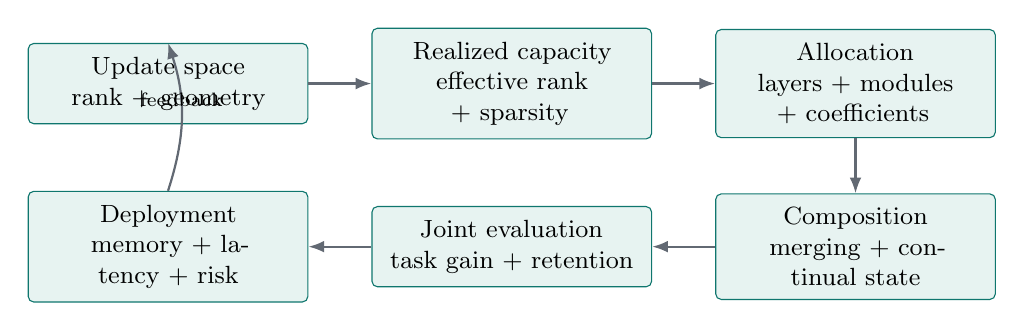
\begin{tikzpicture}[
  node distance=7mm and 8mm,
  box/.style={draw=accent,fill=soft,rounded corners=2pt,align=center,inner sep=5pt,text width=3.2cm,font=\small},
  edge/.style={-{Latex[length=2mm]},thick,draw=ink!70}
]
\node[box] (space) {Update space\\rank + geometry};
\node[box,right=of space] (capacity) {Realized capacity\\effective rank + sparsity};
\node[box,right=of capacity] (alloc) {Allocation\\layers + modules + coefficients};
\node[box,below=of alloc] (merge) {Composition\\merging + continual state};
\node[box,left=of merge] (eval) {Joint evaluation\\task gain + retention};
\node[box,left=of eval] (deploy) {Deployment\\memory + latency + risk};
\draw[edge] (space) -- (capacity);
\draw[edge] (capacity) -- (alloc);
\draw[edge] (alloc) -- (merge);
\draw[edge] (merge) -- (eval);
\draw[edge] (eval) -- (deploy);
\draw[edge,bend right=18] (deploy.north) to node[above,font=\scriptsize]{feedback} (space.north);
\end{tikzpicture}
\caption{Analytical framework used to compare the ten papers. The literature increasingly treats effective capacity and allocation as the causal intermediate variables between parameterization and deployment outcomes.}
\label{fig:map}
\end{figure}

\section{Cross-Paper Synthesis}

\subsection{Explicit geometric preservation is not the main causal factor}

P1 provides the strongest challenge to method-by-label reasoning. It compares LoRA, DoRA, PiSSA, MiLoRA, OFT, and HRA on Qwen2.5-7B, Llama-3.1-8B, and a 4B diffusion model, with method-specific learning-rate search and three seeds. All six methods approximately preserve hyperspherical energy, and the LoRA-family methods also exhibit modest singular-value drift. Restoring pretrained singular values while keeping adapted singular bases changes task performance by less than one percentage point at the largest tested capacities. Therefore, explicitly enforcing spectral preservation is not necessary to preserve task gains in those settings.

What does remain consequential is functional spectral location. Restoring dominant components produces the largest average reduction in general-text NLL or image drift, even when another edit has a larger norm. This result is more useful than the claim that one parameterization is intrinsically orthogonal: forgetting is coupled to changes in dominant pretrained components, while task adaptation can occur through multiple spectral routes.

P1 also shows that method rankings are not stable by metric. LoRA has the lowest mean forgetting in 9 of 12 settings. DoRA leads in 10 of 14 task-score comparisons but may pay additional retention cost. PiSSA often improves task scores yet forgets more: on Qwen2.5-7B coding, its $10^3\Delta\mathrm{NLL}$ is 4.25 versus 1.60 for LoRA; on Llama-3.1-8B it is 43.00 versus 10.73. The practical implication is not ``PiSSA is bad,'' but that a method should be chosen by the task-retention point it occupies.

\subsection{Forgetting explanations currently disagree}

P2 proposes a compact geometric law
\begin{equation}
F=\alpha(1-\cos^2\theta_{\min})+\beta,
\label{eq:angle}
\end{equation}
where $\theta_{\min}$ is the minimum principal angle between task-gradient subspaces. In its controlled synthetic setting the relation reaches $r=0.994$, and forgetting is nearly rank-invariant at high angles. The real-data coefficient of variation is, however, 10--19\%, much larger than the synthetic 0.8\%. The author explicitly labels the angular relation an empirically parameterized regularity rather than a fully derived law.

There is a deeper interpretive problem. The paper reports that greater subspace separation correlates with greater forgetting in its experimental regime, whereas many orthogonal continual-learning methods assume separation should protect prior tasks. P2 argues that the result captures interference under the chosen task-diversity protocol and that explicit orthogonality helps mainly when natural task subspaces overlap. This may be defensible, but it means Eq.~\eqref{eq:angle} cannot be exported as a universal sign prediction. P3 reaches a different practical conclusion: increasing update flexibility reduces interference on its visual task sequence, while severely constraining updates to shared principal directions worsens forgetting. Its ViT-Base results report average forgetting 0.149 for LoRA, 0.209 for PiSSA, and 0.075 for WeGeFT. The discrepancy with P2 is informative: the effect of rank and orthogonality depends on task similarity, parameterization, and whether the adapter uses or disrupts pretrained directions.

P4 supplies a complementary mechanism. LoRA factors are non-identifiable: for any invertible $R$, $BA=(BR)(R^{-1}A)$. Sequentially merging independently optimized factors can therefore compare incompatible latent coordinates. \method{SOAR} constrains $A$ to a Stiefel manifold and aligns $B$ with an orthogonal Procrustes rotation before rank-wise, forgetting-aware merging. On Qwen3-8B, it reaches average accuracy 89.48, 70.96, and 51.59 on three continual benchmarks, versus 85.99, 68.49, and 47.84 for the strongest prior single-adapter baseline, SLAO. The conceptual lesson is stronger than the numerical margin: some observed ``task conflict'' is coordinate-system noise introduced by the parameterization and merging rule.

P9 offers a different theoretical route through maximum-margin classification. Its analysis predicts that LoRA regularization trades the margin on pretrained data against the margin on fine-tuning data, and yields closed-form merging coefficients. Yet its empirical gain is modest: average normalized accuracy is 93.32\% versus 93.15\% for task arithmetic, with a 2.35\% merge-selection runtime overhead. The contribution is explanatory rather than decisively state of the art. Its near-orthogonal-task and linear-classifier assumptions also limit transfer to generative LLM adaptation.

\subsection{Rank increases learning but not automatically retention}

P5 gives the clearest diagnosis of the capacity problem. Standard LoRA reaches only about 361 effective-rank units in a 896-rank mixed-domain setup. The effective-rank utilization falls as the nominal rank grows and is uneven across depth. A Rényi-2 regularizer raises realized rank and improves the learning--retention frontier: on Qwen2.5-0.5B, $\lambda=0.1$ changes training perplexity from 4.77 to 4.53 and Wiki perplexity from 19.60 to 14.65. Across Qwen2.5-0.5B, Qwen2.5-3B-Instruct, and Llama-3.2-3B-Instruct, $\lambda=0.01$ lowers mean Wiki perplexity at every tested rank of at least 16.

This is strong evidence that nominal rank is a poor control variable. It is not, however, a clean causal identification. The authors' norm-bounded alternative also improves the same frontier, so effective-rank maximization cannot be fully separated from norm control. Moreover, most multi-seed evidence centers on the 0.5B model; several high-rank and alternative-method endpoints are single runs. The right engineering claim is therefore conditional: \emph{when rank is introduced as a capacity knob, an underutilized high-rank adapter may be less useful than a smaller update whose singular-value mass is broadly distributed.}

P10 radicalizes this conclusion. Instead of learning both low-rank factors, it freezes an activation-derived input basis and random output dictionaries and learns only scalar coefficients. On Qwen2.5-7B and Llama-3-8B, \method{SCALAR} approaches rank-8 LoRA accuracy using roughly 4\% of LoRA's trainable parameters. Its Qwen2.5-7B commonsense average is 88.9 versus 88.8 for LoRA; peak memory is 49.7 GB versus 62.2 GB, and throughput is 9163 versus 8632 tokens/s. A learned-direction reweighting diagnostic similarly recovers almost all LoRA performance with 196 coefficients rather than 2.52 million parameters.

P10 is a serious challenge to the assumption that both LoRA factors must be optimized. Its limits are equally important. The informative basis is calibrated from downstream activations, so the method assumes access to a representative task distribution. The accuracy differences are often within across-run noise, and fixed-basis storage is reported separately from trainable parameters. Its result may indicate that pretrained models already contain abundant useful perturbation directions; it does not prove that a random basis is universally sufficient.

\subsection{Capacity should be allocated where the task is processed}

P7 provides mechanistic evidence for a layer-efficient alternative. On Qwen2.5-0.5B, path patching attributes 58.4\% of the measured adaptation effect to MLP mediation and 41.6\% to attention; within attention, the value projection accounts for about 46\%, versus 27\% each for query and key. Important layers have only 39.5\% average pairwise Jaccard overlap across four tasks, and only the first three layers are universally selected. Consequently, a global all-layer recipe conflicts with measured task dependence.

\method{Adaptive-LoRA} uses frozen-base zero-ablation to select layers before training. At rank 16 on Qwen2.5-1.5B, adapting 8 of 28 layers yields 59.1\% average commonsense accuracy versus 56.9\% for all-layer LoRA, while using about 3.5 times fewer adapter factors. Across the supplementary three-run study, gains over full-layer LoRA are positive on Qwen2.5-3B and Qwen2.5-7B, nearly neutral on Qwen3-8B (+0.17 points), and mixed on Qwen3-32B outside the relevant size range.

The causal interpretation is not yet settled. Path patching measures mediation through a frozen base model, while LoRA can alter the computation that later layers mediate. The main table uses seed 42; only selected configurations receive three-run validation. The method also selects layers once and keeps them fixed. These issues do not erase the result, but they limit the conclusion to ``task-specific layer selection is a promising capacity-allocation rule,'' not ``30\% is the correct budget.''

\subsection{Small models require a stability screen, not a universal threshold}

P6 studies five models from 135M to 2B. Full fine-tuning becomes unstable below roughly 500M parameters, whereas LoRA and DoRA remain trainable. On Qwen2.5-0.5B, full fine-tuning reaches 0.00\% on SVAMP while LoRA reaches 1.00\%; on SmolLM2-135M, even five-shot in-context learning outperforms the full fine-tuning result.

The paper's practical message -- use PEFT as a default stability screen for small aligned models -- is sensible. Its stronger claim of a 500M ``stability cliff'' is under-supported: only five architectures are tested, each task is represented by one benchmark suite, and PEFT itself is not uniformly beneficial. On Qwen2.5-0.5B, LoRA's SVAMP score of 1.00 remains below the 2.33 zero-shot baseline. The failure is not merely full fine-tuning versus LoRA; it is also task transfer under a narrow 10K-example OrcaMath training set. A threshold should therefore be treated as a hypothesis to test per architecture and data distribution.

P6 also reports an important systems reversal: on eight H100s, full fine-tuning takes 10,289 seconds for Qwen2.5-0.5B, while LoRA takes 19,336 and DoRA 25,960. PEFT is a memory-access and stability strategy, not automatically a wall-clock win when dense kernels and cluster bandwidth are abundant. On consumer hardware, the lower memory footprint can still change feasibility and cost.

\subsection{Additive gains can be mistaken for conditional intelligence}

P8 tests whether input-conditioned adaptation actually uses the current input or merely adds a useful learned correction. With frozen IA3, LoRA, and DoRA adapters, it compares a current-prefix controller with a learned-global controller of equal architecture and nominal parameters. Current-prefix control improves all six mean accuracies over frozen adapters, but no paired contrast with the global control excludes zero. Replacing the current correction with its training-prefix mean changes accuracy by at most 0.34 points; input-varying corrections contribute only 1.8--2.8\% of correction RMS. On the separate ARC test, frozen-adapter current and global controls score 25.68\% and 25.77\%.

This is a model of critical experimental design. It shows that a positive result over a static adapter does not establish that input matching is responsible. The paper does not conclude that all conditional PEFT is ineffective; it concludes that the causal benefit must be isolated. Future gating, routing, and hypernetwork papers should use this matched-control protocol.

\section{Comparative Evidence and Critical Assessment}

\begin{table}[t]
\centering
\caption{Headline evidence and corresponding caveats. Percentages are reported as in the source paper and are not directly comparable across different benchmarks.}
\label{tab:results}
\scriptsize
\begin{tabularx}{\textwidth}{@{}p{0.05\textwidth}p{0.28\textwidth}X X@{}}
\toprule
\textbf{ID} & \textbf{Main quantitative signal} & \textbf{Best-supported interpretation} & \textbf{Principal limitation} \\
\midrule
P1 & LoRA lowest forgetting in 9/12 settings; DoRA best mean task score in 10/14; PiSSA has higher retention cost & Parameterization labels hide a task--retention trade-off; dominant spectral edits matter & Mostly 7B--8B; some synthetic/vision settings; preprint \\
P2 & Synthetic angle law $r=0.994$; real rank-invariance CV 10--19\% & Geometry matters, but the sign and magnitude are regime dependent & Angular model partly empirical; small vision/encoder models \\
P3 & ViT-Base forgetting: LoRA 0.149, PiSSA 0.209, WeGeFT 0.075 & Update parameterization and flexibility matter for retention & Vision only; limited uncertainty reporting \\
P4 & Qwen3-8B averages 89.48/70.96/51.59 over three CL suites & Coordinate alignment improves constant-memory continual LoRA & Fixed training setup; 15.6\% runtime overhead; classification benchmarks \\
P5 & Wiki PPL 14.65 with eRank maximization vs 19.60 for LoRA; eRank 361/896 without penalty & Realized capacity is a better knob than nominal rank & Norm-control confound; uneven seeds and single-run endpoints \\
P6 & Tiny models unstable under full FT; LoRA slower but more feasible on commodity memory & PEFT is a stability and access mechanism for small models & Small model/task sample; ``500M cliff'' is overgeneralized \\
P7 & MLP mediation 58.4\%; task-layer Jaccard 39.5\%; 59.1 vs 56.9 at 30\% layers & Adapt task-selected layers rather than every layer uniformly & Main result one seed; path patching on frozen base \\
P8 & Current/global ARC test 25.68/25.77; varying correction RMS 1.8--2.8\% & Positive gains over static adapters do not prove input conditioning & Mostly small GPT-2/Pythia/Qwen backbones; preprint \\
P9 & Merged normalized accuracy 93.32\% vs 93.15\% for TA & Margins explain merging and give principled coefficients & Linear/near-orthogonal theory; modest empirical lead \\
P10 & 88.9 vs 88.8 average; 20\% lower memory; 6\% higher throughput; ~4\% of LoRA parameters & A small learned coefficient state can retain most adaptation quality & Task-calibrated basis; parity often within noise; preprint \\
\bottomrule
\end{tabularx}
\end{table}

Table~\ref{tab:results} exposes a recurring pattern: the most defensible contributions are mechanisms or evaluation corrections, not universal Pareto improvements. P4, P7, and P10 show material parameter reductions, but each depends on a discovered structure: factor alignment, task-specific layers, or an activation-derived basis. P5 shows that a higher nominal rank is not automatically better. P1 and P8 show that careful controls can erase or reframe apparent gains. These are not contradictory outcomes; they define the conditions under which each method should be expected to work.

\subsection{Model scale and external validity}

Most reliable evidence lies between 0.5B and 8B parameters. This is the right regime for the assignment's deployment constraint, but it creates two risks. First, a method that wins at 1.5B may be solving a parameter-scarcity problem that disappears at 30B. Second, a method evaluated only at 7B may depend on layer count, hidden width, or an unusually well-aligned instruction model. The reviewed papers rarely test an explicit scaling curve for their mechanism. P7 reports a neutral Qwen3-8B result and mixed evidence at 32B; P5 finds different gains across models; P1 shows backbone-dependent task and retention ordering. The safe conclusion is therefore a set of conditional hypotheses, not fixed hyperparameters.

\subsection{Benchmark and metric threats}

Commonsense averages are dominated by eight multiple-choice tasks, while coding is represented by HumanEval and MBPP. These benchmarks do not test long-context use, dialogue, tool use, multilingual transfer, or refusal behavior. Retention is often measured by perplexity on a small general-text corpus, which is insensitive to alignment failure. P6 even reports catastrophic behavioral collapse that is only indirectly visible in the chosen metrics. A deployment-oriented study should add calibration error, safety-refusal consistency, hallucination rate, and task-specific failure analysis.

The papers also use different parameter budgets. P10 reports a very small trainable state but also fixed basis storage. P5 uses maximal rank 896 or 3072 on some models, which is far above common LoRA practice. P7 compares selected layers at the same rank, while P4 uses rank 32. ``Parameter efficiency'' can therefore refer to trainable parameters, adapter checkpoint size, activation memory, or wall-clock throughput. These quantities must be reported separately.

\subsection{Statistical and causal threats}

Several headline claims are based on one seed. P1, P8, and P9 are comparatively strong because they use multiple seeds and interventions. P7 improves on this by adding a three-run appendix, but its main 11-task table remains single-seed. P5 and P10 use three repeated runs for core comparisons, yet important robustness cases are single-run. Confidence intervals are often absent or are bootstrap intervals over few training seeds. A method difference smaller than one standard deviation should not be presented as a stable ranking.

Causal language is also uneven. P1 directly edits singular components; P8 directly replaces input-varying corrections; P7 path-patches components. These designs support stronger claims than a post-hoc correlation between rank and forgetting. P2's geometric fit, for example, is a regression over task regimes rather than a controlled intervention on angle. P3's comparison of parameterizations is controlled but vision-specific. A future paper should combine prospective geometric measurement, randomized intervention, and multi-seed downstream evaluation.

\subsection{Reliability and practical risk}

LoRA variants can reduce the cost of adaptation but do not guarantee safe adaptation. None of the ten papers systematically evaluates whether a smaller adapter preserves safety alignment, memorization behavior, or privacy after domain training. A compact adapter may forget less general knowledge while still changing refusal behavior on a narrow class of prompts. The community should treat task performance, general retention, and safety behavior as a three-dimensional evaluation problem.

\section{Research Agenda for Sub-30B Adaptation}

\subsection{A controlled benchmark protocol}

The field would benefit from a shared benchmark that I will call \emph{SPARE-30} (Stability-Preserving Adaptation and Retention Evaluation under 30B). The protocol should include:
\begin{enumerate}
  \item \textbf{Model ladder:} at least three families and approximate sizes at 1B, 3B, 7B, and 13B, with one 30B endpoint when hardware permits.
  \item \textbf{Matched budgets:} separate comparisons at equal trainable parameters, equal adapter storage, equal peak memory, equal optimizer steps, and equal wall-clock time.
  \item \textbf{Tuning:} method-specific learning-rate search on a development split, followed by at least five training seeds.
  \item \textbf{Adaptation suite:} math, code, instruction following, classification, and one long-context task.
  \item \textbf{Retention suite:} general-text likelihood, held-out reasoning, calibration, safety refusals, and knowledge probes.
  \item \textbf{Mechanistic diagnostics:} nominal and effective rank, singular-vector drift, gradient-subspace angle, layer contribution, and adapter checkpoint size.
  \item \textbf{Release:} scripts, exact budgets, hardware, failed runs, and final adapters.
\end{enumerate}

\subsection{Research questions that follow from the evidence}

\paragraph{Capacity law.}
Can realized effective rank, gradient-subspace angle, and norm control be combined into a predictive model of the adaptation--retention frontier? P5 suggests that rank utilization matters; P2 and P3 show that geometry changes the sign of the effect. A useful law must predict the boundary between learning and interference rather than fit one dataset.

\paragraph{Prospective layer allocation.}
P7 shows that layer importance is task-specific. Future work should ask whether a tiny calibration set can reliably predict layer budgets for unseen tasks, whether selection should adapt during training, and whether the result transfers to generative tasks. The main comparison should be against gradient-guided and random layer selection at the same memory cost.

\paragraph{Factor-free and coefficient-only adaptation.}
P10 demonstrates that many useful directions may already exist around pretrained weights. Future work should test whether task-calibrated bases can be obtained without task labels, how they behave under distribution shift, and whether compact coefficients can be merged or continually updated without catastrophic coordinate drift.

\paragraph{Identification-aware continual learning.}
P4 and P9 indicate that part of adapter merging is a latent-coordinate problem. A unified study should separate parameterization non-identifiability from genuine task conflict by using interventions that fix $BA$ while varying $(B,A)$. If accuracy changes under equivalent factorizations, the merge rule is not measuring the intended object.

\paragraph{Input-conditioned control with causal tests.}
P8 provides a template. A new gating or routing method should beat an equal-parameter learned-global baseline, not merely a static adapter. It should also report the fraction of correction energy that actually varies with input and the result of replacing that variation with a fixed mean.

\paragraph{Hardware-aware model economics.}
P6 shows that PEFT can be slower on a cluster. P10 shows gains in memory and throughput on a particular hardware stack. Future evaluations should report tokens per second, peak memory, energy, optimizer-state size, and inference latency, not just ``trainable parameter percentage.''

\section{Conclusion}

The 2026 literature does not support a simple winner among LoRA, DoRA, PiSSA, fixed-basis adaptation, or layer-selective adaptation. It supports a more operational conclusion: adaptation quality depends on where a model spends update capacity, how much capacity the optimizer actually uses, and which pretrained directions are disturbed. Nominal rank oversimplifies all three. Explicit orthogonality can be helpful, irrelevant, or even counterproductive depending on task geometry. Additional trainable parameters can improve fitting while worsening retention. Small adapters can preserve general likelihood while still changing safety behavior.

For models below 30B, the most defensible practical strategy is staged rather than universal. Start with a stability check on the target small model, tune LoRA or a compact coefficient method under an equal-memory budget, measure effective rank and layer sensitivity, and evaluate task gain jointly with general retention and safety. If multiple tasks must coexist, treat adapter alignment as part of the learning problem rather than a post-hoc averaging step. If a proposed method claims input-adaptive intelligence, isolate its gain against a learned-global control. These steps are modest, but they directly address the contradictions visible in the current literature.

\appendix
\section{Screening Notes and Assessment Checklist}

\subsection{Why these ten papers were retained}

The final set deliberately balances four kinds of evidence: theory with prediction (P2, P9), controlled empirical comparison (P1, P3, P8), mechanistic and allocation studies (P7), and deployment-oriented compact adaptation (P4, P5, P6, P10). This mix prevents the review from becoming a catalogue of parameter-reduction methods. P1 and P8 serve as adversarial checks on the other papers: they show which claims require stronger controls. P5, P7, and P10 provide the strongest practical clues for sub-30B deployment. P2, P3, and P4 identify the unresolved geometry of forgetting.

\subsection{Questions to ask when interpreting a paper}

\begin{enumerate}
  \item Is the reported rank the configured rank or the effective rank?
  \item Are adapters compared at equal trainable parameters, equal checkpoint storage, equal memory, or equal compute?
  \item Were learning rates tuned separately for each method on a development split?
  \item How many training seeds and task orders were used?
  \item Does the retention metric include behavior and safety, or only general-text likelihood?
  \item If the method claims input dependence, is there an equal-parameter learned-global control?
  \item Are results below 30B reported separately from larger-model extrapolations?
  \item Are failed runs, calibration data, fixed bases, and inference overhead disclosed?
\end{enumerate}

\section*{References}
\begin{thebibliography}{99}
\small

\bibitem{li2026different}
Y. Li, P. Lu, and F. Liu.
\newblock Are Parameter-Efficient Fine-tuning Methods Really Different?
\newblock arXiv:2610.09122, 6 October 2026.
\newblock \url{https://arxiv.org/abs/2610.09122}

\bibitem{steele2026subspace}
B. Steele.
\newblock Subspace Geometry Governs Catastrophic Forgetting in Low-Rank Adaptation.
\newblock arXiv:2603.02224, 10 February 2026.
\newblock \url{https://arxiv.org/abs/2603.02224}

\bibitem{ahmad2026forgetting}
M. Ahmad, J. Zheng, and Y. Cao.
\newblock On Catastrophic Forgetting in Low-Rank Decomposition-Based Parameter-Efficient Fine-Tuning.
\newblock arXiv:2603.09684, 10 March 2026.
\newblock \url{https://arxiv.org/abs/2603.09684}

\bibitem{singh2026soar}
P. R. Singh, M. Zaki, A. Saha, A. Mukkamala, and P. Wasnik.
\newblock Making LoRA Identifiable: Orthogonal Alignment for Continual Learning.
\newblock NeurIPS 2026. arXiv:2610.16664.
\newblock \url{https://arxiv.org/abs/2610.16664}

\bibitem{sawada2026capacity}
T. Sawada and K. Goyal.
\newblock Maximizing Capacity Utilization of LoRA Adapters for Mitigating the Learning-Forgetting Trade-off.
\newblock arXiv:2611.17191, 12 November 2026.
\newblock \url{https://arxiv.org/abs/2611.17191}

\bibitem{nair2026trap}
R. Nair and C. Tao.
\newblock The Fine-Tuning Trap: Evaluating Negative Transfer and the Role of PEFT in Sub-1B Mathematical Reasoning.
\newblock arXiv:2606.06920, 5 June 2026.
\newblock \url{https://arxiv.org/abs/2606.06920}

\bibitem{zuo2026mechanistic}
F. Zuo, Y. Huang, and K. Wang.
\newblock Mechanistic Insights into LoRA: Layer Sparsity for Adaptive Fine-Tuning via Path Patching.
\newblock NeurIPS 2026 Main Track. arXiv:2610.34756.
\newblock \url{https://arxiv.org/abs/2610.34756}

\bibitem{yudistira2026preface}
N. Yudistira and O. Octadion.
\newblock PREFACE: Separating Shared Corrections from Prefix Conditioning in PEFT.
\newblock arXiv:2611.18987, 13 November 2026.
\newblock \url{https://arxiv.org/abs/2611.18987}

\bibitem{xu2026malora}
Z. Xu, H. Min, L. E. MacDonald, S. Tarmoun, E. Mallada, W. Su, and R. Vidal.
\newblock A Margin Perspective on LoRA: Robustness to Catastrophic Forgetting and Adapter Merging (MaLoRA).
\newblock NeurIPS 2026. arXiv:2611.14397.
\newblock \url{https://arxiv.org/abs/2611.14397}

\bibitem{wen2026scalar}
Z. Wen, X. Song, J. Wang, P. Luo, J. Zeng, D. Li, K. Xu, and T. Sun.
\newblock Direction or Magnitude? Learning Scalars over Task-Calibrated Directions.
\newblock arXiv:2611.17784, 13 November 2026.
\newblock \url{https://arxiv.org/abs/2611.17784}

\end{thebibliography}

\end{document}
